\documentclass{article}

\usepackage[utf8x]{inputenc}
\usepackage[finnish]{babel}
\usepackage{hyperref}
\usepackage{graphicx}
\usepackage{float}
\usepackage{enumitem}

\setlength{\parindent}{0.0in}
\setlength{\parskip}{0.1in}

\let\stdsection\section
\renewcommand\section{\newpage\stdsection}

\begin{document}
\title{Aineopintojen harjoitustyö: Tietokantasovellus \\ Twitter-kloonin dokumentaatio}
\author{Mika Viinamäki}
\maketitle
\thispagestyle{empty}

\newpage

\tableofcontents
\newpage

\section{Johdanto}

\subsection {Järjestelmän tarkoitus}
Järjestelmän tarkoitus on olla yksinkertainen kopio Twitterin tarjoamasta mikroblogista. Käytännössä käyttäjät voivat lähettää enintään 140 merkin pituisia viestejä omalle sivulleen ja halutessaan lisätä niihin "hashtageja" lisäämällä jonkin viestin sanan eteen \verb+#+-merkin tai viittauksia muihin palvelun käyttäjiin lisäämällä käyttäjätunnuksen eteen \verb+@+-merkin.

Käyttäjä pystyy myös seuraamaan muita käyttäjiä, jolloin niiden viestit näkyvät omalla sivulla. Myös viestit, joissa käyttäjää on viitattu, näkyvät samalla sivulla -- tämä toiminnallisuus eroaa jonkin verran Twitterin vastaavasta.

\subsection{Toimintaympäristö}
Järjestelmä on toteutettu Pythonilla Linux-ympäristössä käyttäen apuna Flask-sovelluskehystä, ja vaatii siis toimiakseen Pythonia tukevan ympäristön. Tietokantanaan se pystyy käyttämään ainakin SQLite:a ja PostgreSQL:aa, todennäköisesti muutkin järjestelmän käyttämän SQLAlchemy-kirjaston tukemat tietokannat toimivat.

Järjestelmä on suunniteltu toimimaan Heroku-palvelussa suoraan. Testiasennus löytyy osoitteesta \url{http://tsoha-toot.herokuapp.com}. Testaamista varten voi rekisteröityä palveluun, sähköpostiosoitteiden ei tarvitse olla oikeita.

\subsection{Rajaukset}
Järjestelmään ei varmaankaan tulla toteuttamaan mitään ylläpitotoimintoja.

\section{Yleiskuva järjestelmästä}

\subsection{Sidosryhmäkaavio}

\begin{figure}[H]
    \centering
    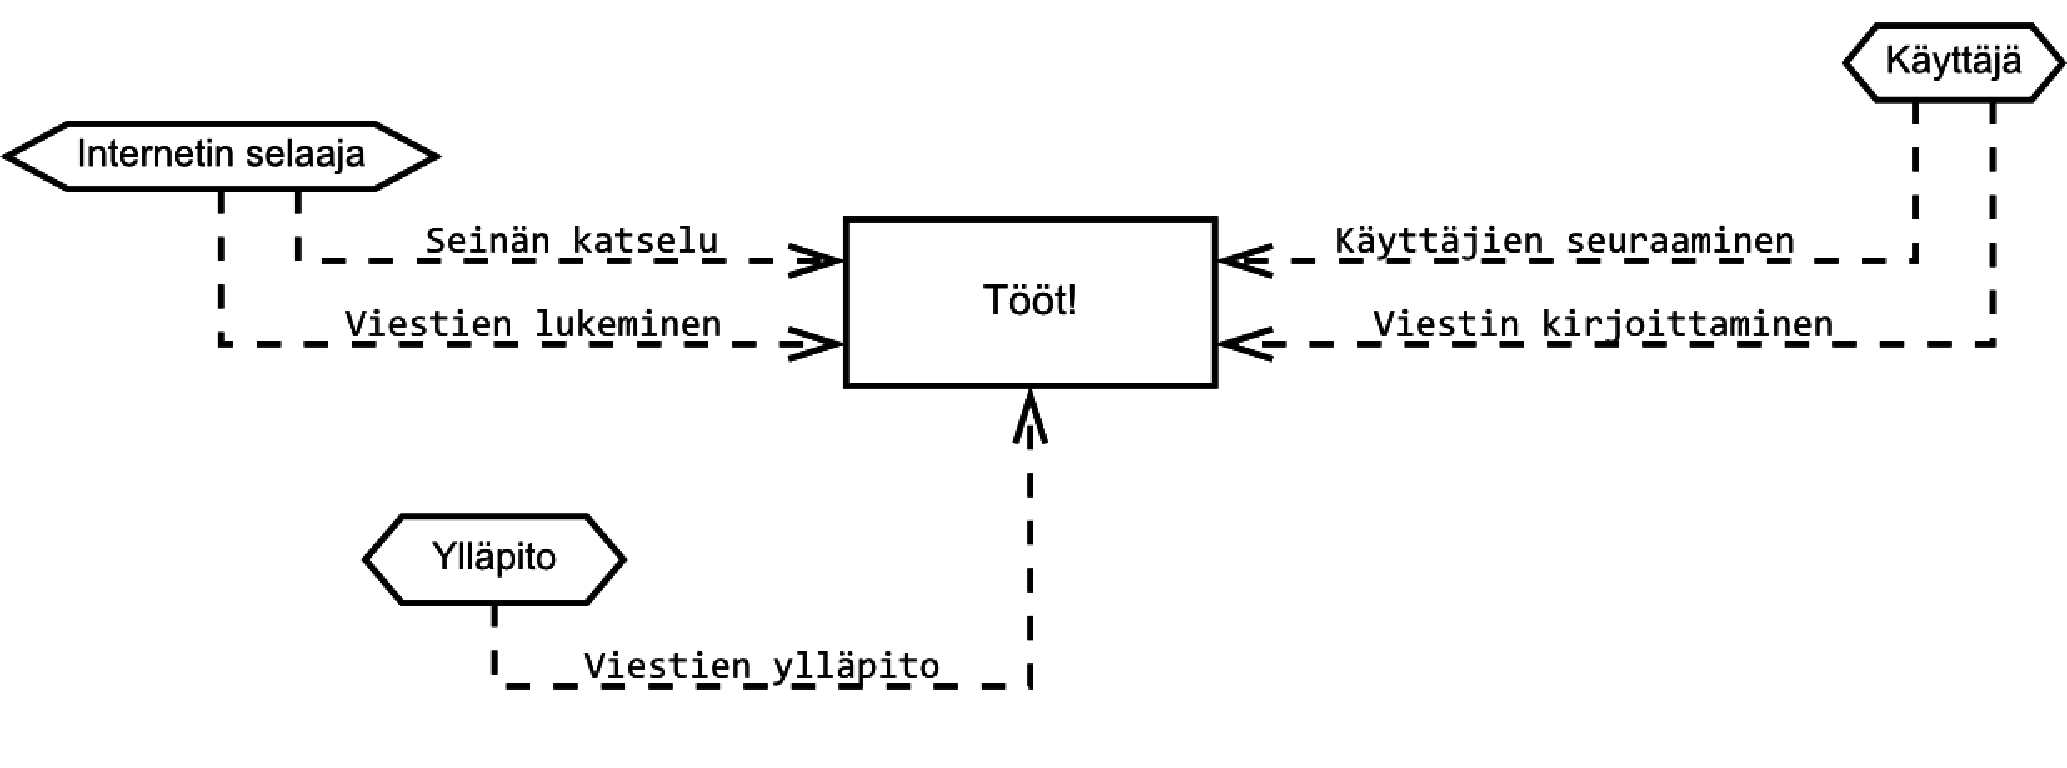
\includegraphics[width=\textwidth]{sidosryhmat.pdf}
\end{figure}

\subsection{Käyttäjäryhmät}

\begin{description}
    \item[Internetin selaaja] Satunnainen, sivulle jostain syystä eksynyt internetin käyttäjä, joka on kiinnostunut käyttäjien kirjoittamista viesteistä.    
    \item[Käyttäjä] Palveluun rekisteröitynyt käyttäjä, joka haluaa lähettää palveluun viestejään.
    \item[Ylläpito] Palvelun toiminnasta huolehtivat henkilöt.
\end{description}

\section{Käyttötapaukset}

\subsection{Internetin selaaja}

\subsubsection{Käyttäjän viestien katseleminen}
Kuka tahansa voi katsella jonkun tietyn käyttäjän lähettämiä viestejä.

\subsubsection{Käyttäjän seinän katseleminen}
Kuka tahansa pystyy katselemaan kenen tahansa käyttäjän seinää, jossa näkyy käyttäjän seuraamien käyttäjien lähettämät viestit ja viestit, jossa kyseinen käyttäjä on mainittu.

\subsubsection{Tietyn hashtagin sisältävien viestien katseleminen}
Kuka tahansa pystyy katselemaan viestejä, joissa jokin tietty hashtag on mainittu.

\subsection{Käyttäjä}

\subsubsection{Viestin lähettäminen}
Käyttäjä pystyy lähettämään maksimissaan 140-merkkisen viestin palveluun. Viestissä voi olla hashtageja, linkkejä tai viittauksia muihin palvelun käyttäjiin.

\subsubsection{Käyttäjän seuraaminen ja seuraamisen poistaminen}
Käyttäjä pystyy asettamaan jonkun toisen käyttäjän seuratuksi ja poistamaan seurauksen.

\subsubsection{Oman viestin poistaminen}
Käyttäjä voi poistaa lähettämänsä viestin palvelusta.

\subsection{Ylläpitäjä}
Ylläpitäjältä ei varmaankaan toteuteta mitään käyttötapauksia.

\section{Järjestelmän tietosisältö}

\subsection{Tietosisältökaavio}

\begin{figure}[H]
    \centering
    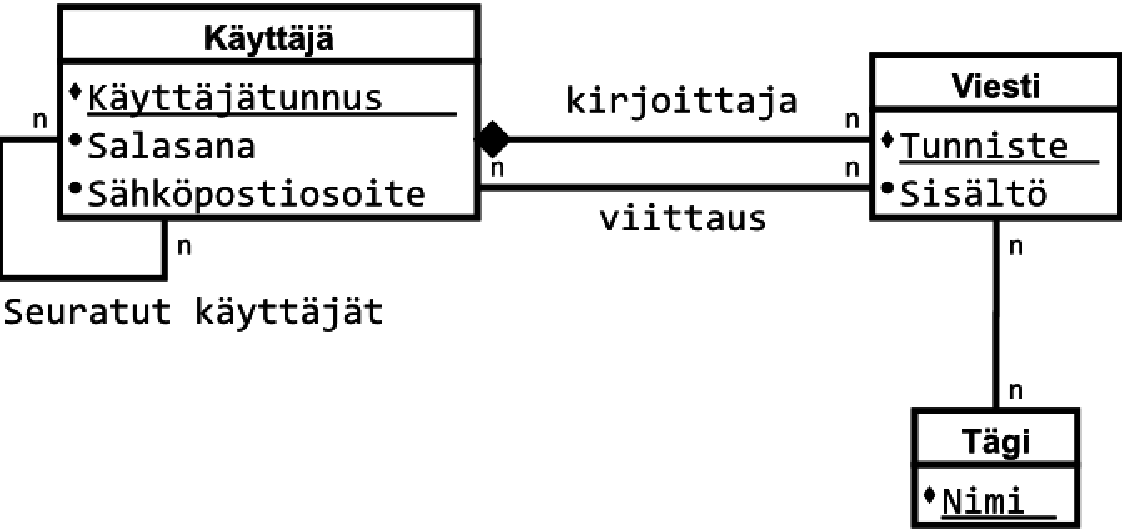
\includegraphics[width=0.8\textwidth]{tietosisalto.pdf}
\end{figure}

\subsection{Tietokohteiden kuvaukset}

\subsubsection{Käyttäjä}

Palveluun rekisteröinyt käyttäjä. Yksi käyttäjä voi olla lähettänyt palveluun useita viestejä. Lisäksi käyttäjään voi liittyä useita muita käyttäjiä, joita hän seuraa.

\begin{description}[itemsep=0pt]
    \item[Attribuutti] Käyttäjätunnus
    \item[Arvojoukko] Pienistä kirjaimista koostuva 6-20 merkkiä pitkä merkkijono.
    \item[Kuvailu] Käyttäjän palvelussa käyttämä uniikki käyttäjätunnus.
\end{description}

\begin{description}[itemsep=0pt]
    \item[Attribuutti] Salasana
    \item[Arvojoukko] Salasanasta muodostettu bcrypt-hash.
    \item[Kuvailu] Käyttäjän kirjautumiseen käyttämä salasana.
\end{description}

\begin{description}[itemsep=0pt]
    \item[Attribuutti] Sähköpostiosoite
    \item[Arvojoukko] Validi sähköpostiosoite merkkijonona.
    \item[Kuvailu] Käyttäjän sähköpostiosoite.
\end{description}


\subsubsection{Viesti}

Käyttäjän palveluun lähettämä viesti. Viesti kuuluu aina jollekin käyttäjälle. Lisäksi viestiin voi liittyä erilaisia tägejä. Lisäksi viestissä voi olla viittaus useaan käyttäjään. Tägit ja viittaukset voidaan päätellä viestin sisällöstä - ne on merkitty sisältöön laittamalla sanan eteen tägin tapauksessa \verb+#+-merkin ja viittauksen tapauksessa \verb+@+-merkin.

\begin{description}[itemsep=0pt]
    \item[Attribuutti] Tunniste
    \item[Arvojoukko] Uniikki numero.
    \item[Kuvailu] Viestin numeromuotoinen yksilöivä tunniste.
\end{description}

\begin{description}[itemsep=0pt]
    \item[Attribuutti] Sisältö
    \item[Arvojoukko] Merkkijono, enintään 140 merkkiä.
    \item[Kuvailu] Viestin sisältö.
\end{description}

\subsubsection{Tägi}

Viestiin liittyvä tägi. Sama tägi voi liittyä useaan viestiin, ja yhteen viestiin voi liittyä useita tageja.

\begin{description}[itemsep=0pt]
    \item[Attribuutti] Nimi
    \item[Arvojoukko] Uniikki, pienistä kirjaimista koostuva, enintään 140 merkkiä pitkä merkkijono.
    \item[Kuvailu] Tägin nimi.
\end{description}

\subsection{Relaatiotietokantakaavio}

\begin{figure}[H]
    \centering
    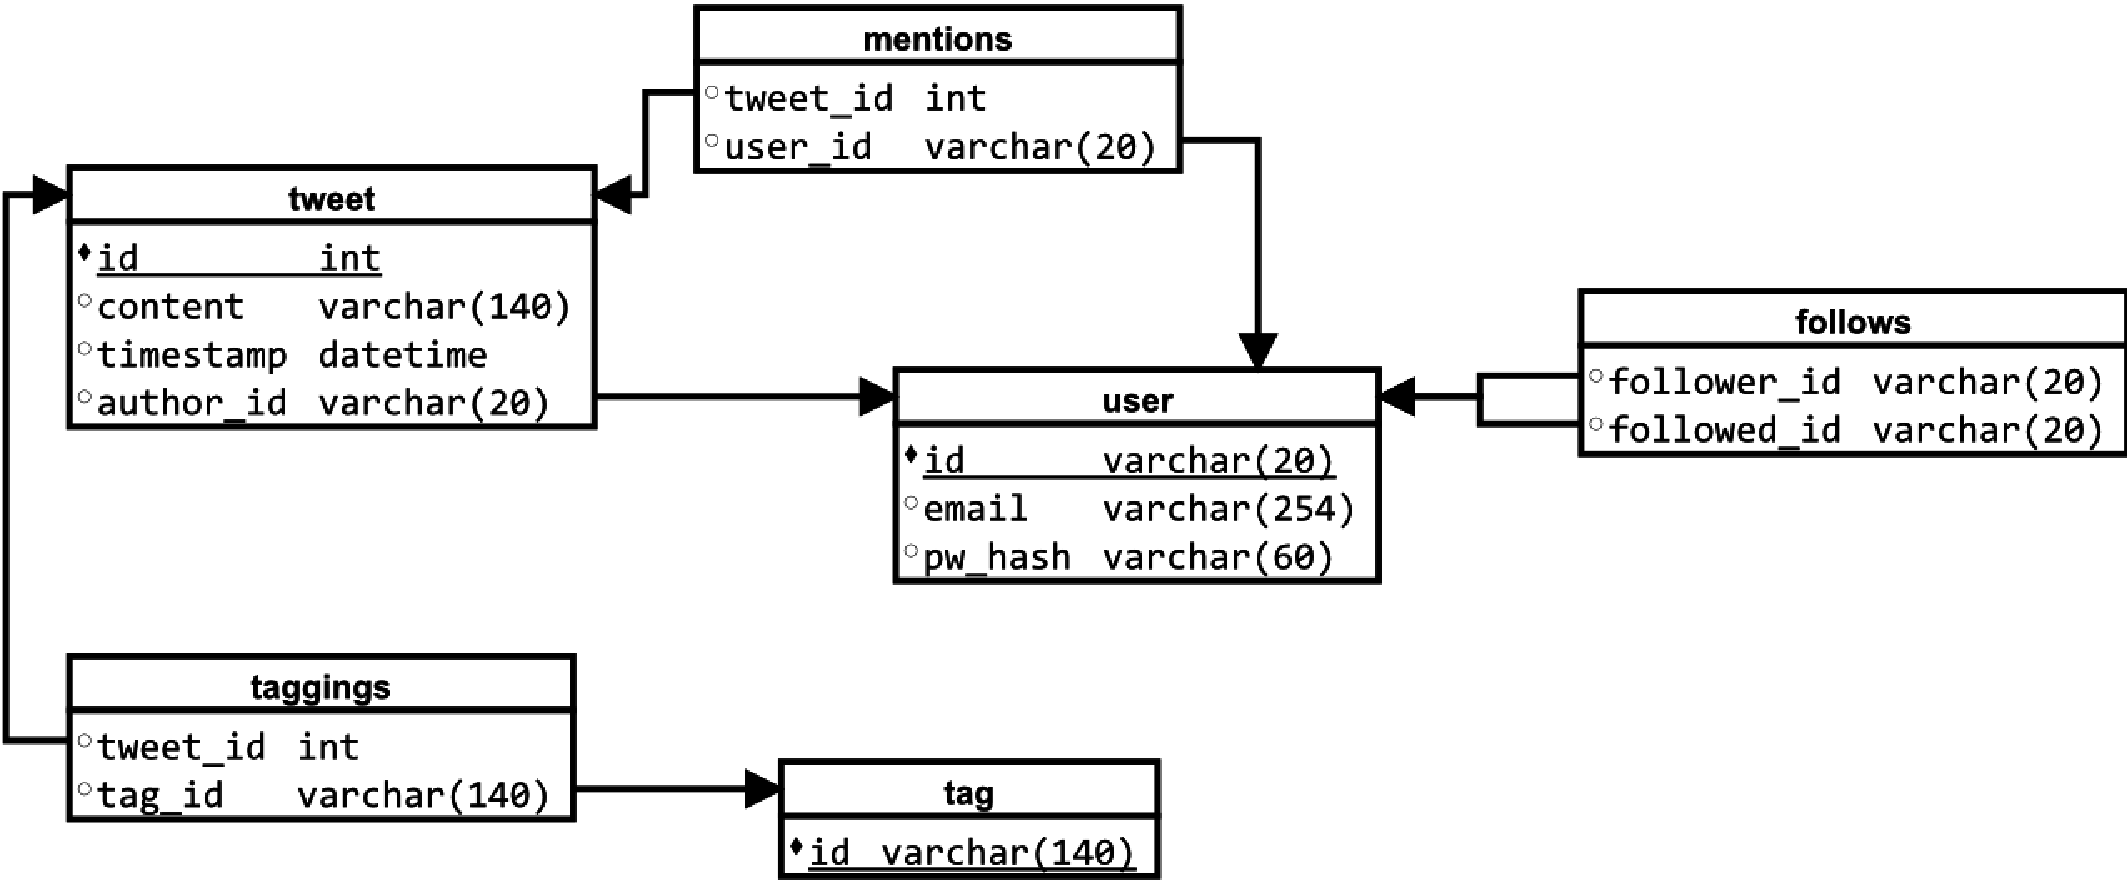
\includegraphics[width=\textwidth]{tietokanta.pdf}
\end{figure}

Ohjelma käyttää SQLAlchemy-kirjaston deklaratiivista tietokannan määrittelyä, jonka avulla pystytään generoimaan SQL-lauseet monille eri tietokantaohjelmistoille -- siispä SQL-lauseita ei ole dokumentissa mukana tai liitteenä.

\section{Järjestelmän yleisrakenne}

\subsection{Projektin tiedostot}

\begin{description}
\item[\texttt{docs/}] Kansio, jossa tähän dokumenttiin liittyvät tiedostot.
\item[\texttt{docs/docs.pdf}] Tämä dokumentti.
\item[\texttt{app/}] Kansio, joka sisältää kaiken ohjelmakoodin.
\item[\texttt{app/initalize\_db.py}] Python-skripti, jolla saa luotua tietokannan.
\item[\texttt{app/static/}] Kansio, joka sisältää kaikki web-sovelluksen staattiset tiedostot - esimerkiksi CSS-tyylitiedostot.
\item[\texttt{app/static/css/bootstrap.min.css}] Bootstrap-kirjasto, jota käytetään sivun ulkoasun pohjana.
\item[\texttt{app/static/css/own.css}] Omat CSS-tyylit.
\item[\texttt{app/templates/}] Kansio, jossa ovat HTML-koodin generoinnissa käytettävät Jinja2-templatet.
\item[\texttt{app/main.py}] Sovelluksen "päätiedosto". Sisältää mm. SQL- ja muut asetukset sekä kaikki näkymät.
\item[\texttt{app/models.py}] Tietokantamallit sisältävä tiedosto.
\item[\texttt{app/forms.py}] Lomakkeet sisältävä tiedosto.
\item[\texttt{Procfile}] Sovelluksen ajamiseen tarvittavat tiedot Herokua varten.
\item[\texttt{requirements.txt}] Sovelluksen tarvitsemat kirjastot.
\end{description}

\subsection{Käyttöliittymäkaavio}
\begin{figure}[H]
    \centering
    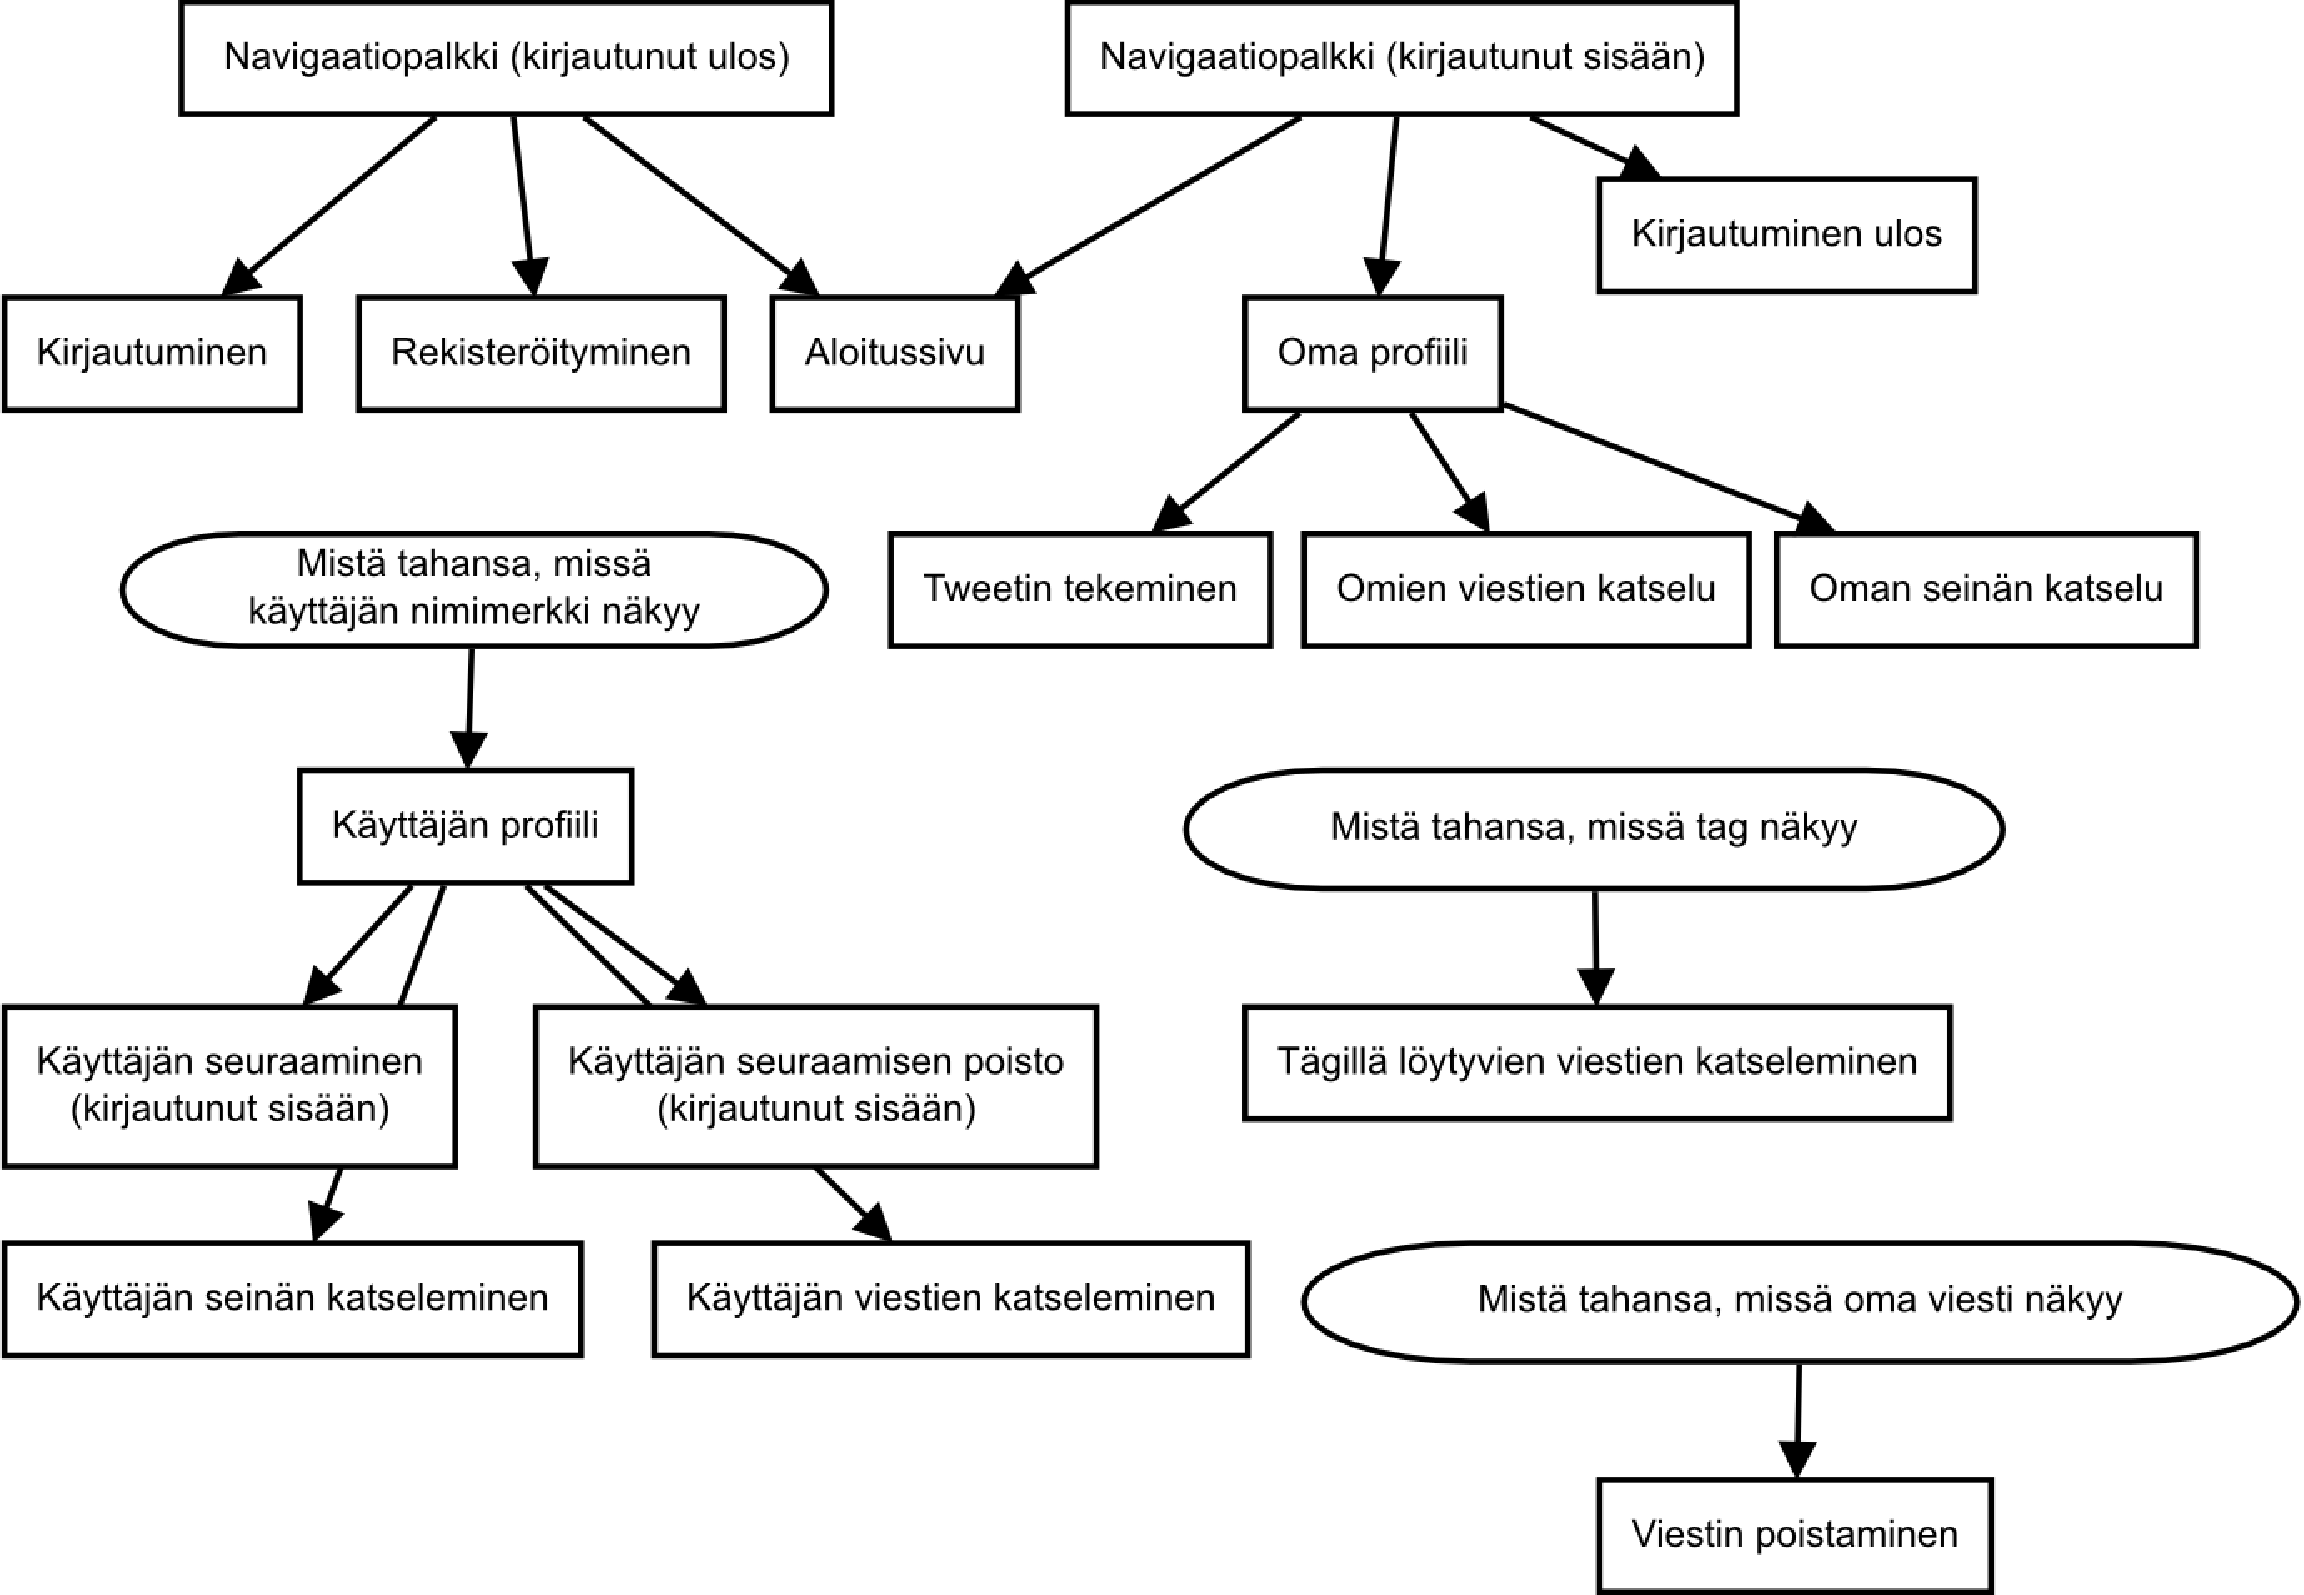
\includegraphics[width=\textwidth]{navigaatio.pdf}
\end{figure}

\section{Asennustiedot}
Ohje olettaa, että käytössä on Linux, Python 2.7 ja virtualenv.

\subsection{Paikallisen version ajaminen}
Ensin kloonataan git-repositorio GitHubista paikalliselle koneelle ja siirrytään kyseiseen repositorioon:

\texttt{\$ git clone git://github.com/Kauhsa/tsoha-toot.git} (tai vaikkapa oman forkin git-osoite) \\
\texttt{\$ cd tsoha-toot}

Luodaan uusi virtualenv - ei pakollista, mutta riippuvuuksien hoitaminen on muuten vaikeaa ainakin ilman root-oikeuksia.

\texttt{\$ mkvirtualenv --python=python2 toot}

Asennetaan ohjelmiston tarvitsemat riippuvuudet.

\texttt{\$ pip install -r requirements.txt}

Luodaan tietokanta, ohjelmisto käyttää oletuksena SQLiteä jos muuta ei määritellä:

\texttt{\$ python app/initialize\_db.py}

Ajetaan kehityspalvelin:

\texttt{\$ python app/main.py}

Nyt palvelimen pitäisi olla päällä, ja sovellukseen pääsee käsiksi selaimella käyttämällä osoitetta \url{http://127.0.0.1:5000/}.

\subsection{Herokuun siirtäminen}

Oletetaan, että Heroku-tunnus on luotu, siihen on kirjauduttu ja Heroku Toolbelt on asennettu.

Luodaan uusi Heroku-applikaatio.

\texttt{\$ heroku create}

Lisätään projektiin tietokanta:

\texttt{\$ heroku addons:add heroku-postgresql:dev} \\
\texttt{\$ heroku pg:promote}

Viedään projekti Herokuun:

\texttt{\$ git push heroku master}

Luodaan tietokanta palvelimelle:

\texttt{\$ heroku run python2 app/initalize\_db.py}

Avataan ohjelma:

\texttt{\$ heroku open}

Web-sovelluksen pitäisi avautua selaimessa.

\end{document}